\section{Multi-layer Perceptron (MLP)}
\label{sec:Multilayer_Perceptro_marker}
\subsubsection{Cenni storici}
I primi tentativi teorici di estendere il perceptron a più livelli 
risalgono agli studi di Ivakhnenko e Lapa negli anni '60 e '70, ma erano 
limitati e computazionalmente costosi. Inoltre, la mancanza di un algoritmo 
efficace per aggiornare i pesi impedì progressi significativi.
Solo verso il 1986 con l'introduzione dell'algoritmo di 
retropropagazione (backpropagation), formalizzato da David Rumelhart, 
Geoffrey Hinton e Ronald Williams nel loro articolo, si aprirono nuove 
possibilità per realizzare queste tipologie di reti \cite{Articolo_backpropagation}.


\subsubsection{Struttura del modello}
l percettrone multistrato è una vera e propria rete neurale artificiale 
composta, come si evince dal nome, da più strati di percettroni. Esso si compone di 
un livello di input, il quale riceve il segnale, ed un livello di output, che esegue 
una previsione o prende una decisione per quanto concerne l’input e, tra 
questi due livelli, vi è un numero arbitrario di strati “nascosti” (hidden), il vero motore 
computazionale della rete. Ciascun neurone di un livello è connesso a tutti i 
neuroni del livello precedente, per tale motivo una rete di questo tipo è anche 
detta Fully Connected 
\cite{ASPETTI_APPRENDIMENTO_PERCETTONE,GradientDescent_NeuralNetworks,ALL_DEEP_LEARNING}. 

\begin{figure}[H]
    \centering
    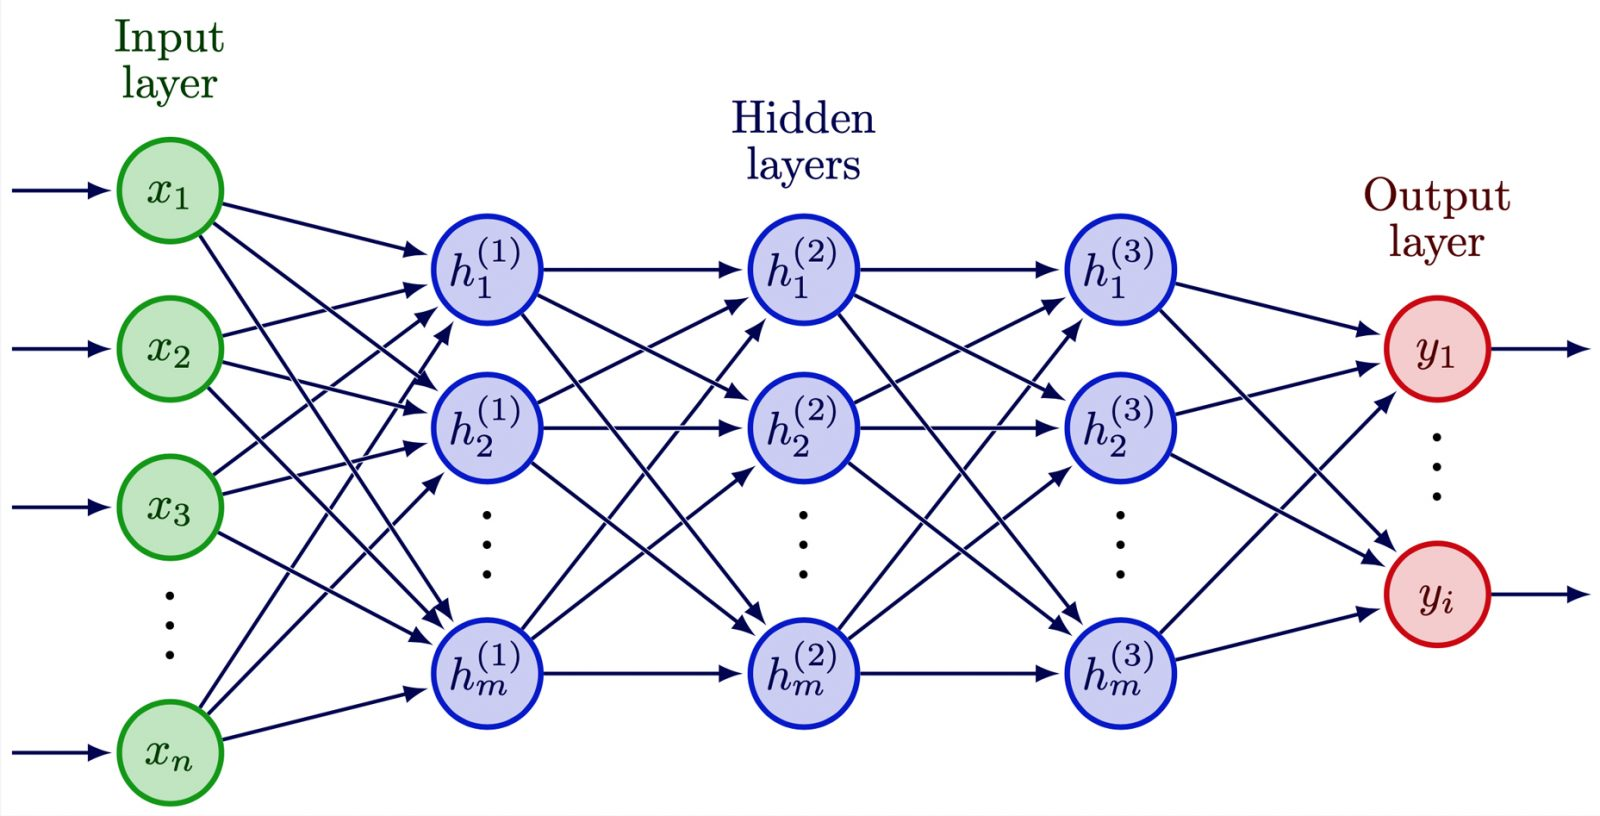
\includegraphics[width=0.8\textwidth]{Immagini/Generiche/MLP_v2.jpg}
    \caption{Esempio di un MLP \cite{Immagine_MLP}.}
    \label{fig:MLP_GRAPH3}
    %Figura 2.1: Esempio schematico di un neurone
\end{figure}

Nel corso dell’ultimo decennio è diventato sempre più frequente l’utilizzo di reti 
neurali aventi molteplici \textit{hidden layer}. Una rete neurale avente più di 
un \textit{hidden layer} è detta anche \textbf{rete neurale profonda (deep neural network)} e l’insieme di queste 
reti costituiscono la base del moderno \textit{deep learning}.
Spesso ci si riferisce a questi modelli anche con \textit{feed forward network}.

\subsection{Rappresentazione matematica del modello}
Un Multi-Layer Perceptron (MLP) può essere formalizzato matematicamente 
come una sequenza di trasformazioni lineari, seguite da funzioni di attivazione 
non lineari. 
\subsubsection{Notazione}
Prima di passare a definire le formule modello, vediamo la notazione
utilizzata dal modello 
\cite{GradientDescent_NeuralNetworks,ALL_DEEP_LEARNING,ASPETTI_MLP_1,ASPETTI_MLP_2}:

\begin{itemize}
    \item Il numero di livelli (o layer) della rete sono denotati con $L$,
    e per riferirsi ad un layer generico, useremo la lettera $l$, con $l\in [0, L]$; 

    \item Con la notazione $n_l$ ci si riferisce al numero di percettroni (o neuroni)
    che compongono un generico livello $l$;

    \item Con $h^{(l)}$ si indica il vettore colonna dei risultati delle funzioni 
    di attivazione calcolate al livello $l$;

    \item Per rappresentare gli input della rete viene utilizzato un vettore colonna di dimensione $d$,
    dove $d$ rappresenta il numero degli input della rete:
    
    \[
        \mathbf{X} = \begin{bmatrix} x_1 \\ x_2 \\ \vdots \\ x_n \end{bmatrix} \in \mathbb{R}^d
    \]

    \item Per rappresentare i pesi di ogni layer $l$, viene utilizzata una matrice $\mathbf{W}^{(l)}$ di dimensioni
    $n_l \times n_{l-1}$, dove $n_l$ è il numero di neuroni nel livello corrente 
    e $n_{l-1}$ è il numero di neuroni nel livello precedente:
    
    \[
        \mathbf{W}^{(l)} = 
        \begin{bmatrix}
        w_{11}^{(l)} & w_{12}^{(l)} & \cdots & w_{1n_{l-1}}^{(l)} \\
        w_{21}^{(l)} & w_{22}^{(l)} & \cdots & w_{2n_{l-1}}^{(l)} \\
        \vdots & \vdots & \ddots & \vdots \\
        w_{n_l1}^{(l)} & w_{n_l2}^{(l)} & \cdots & w_{n_ln_{l-1}}^{(l)}
        \end{bmatrix}
        \in \mathbb{R}^{n_l \times n_{l-1}}
    \]

    In questa matrice, ogni colonna rappresenta i pesi degli input associati a
    un singolo percettrone (o neurone) del layer;
    

    \item Per ogni livello $l$, il bias è rappresentato come un vettore 
    colonna di dimensioni $n_l$:
    
    \[
        \mathbf{b}^{(l)} = 
        \begin{bmatrix}
        b_1^{(l)} \\
        b_2^{(l)} \\
        \vdots \\
        b_{n_l}^{(l)}
        \end{bmatrix}
        \in \mathbb{R}^{n_l}
    \]

    \item Per denotare la funzione di attivazione usata al livello $l$, si
    utilizza la notazione $\boldsymbol{\sigma^{(l)}}$. Pertanto, ogni percettrone (o neurone) 
    del livello $l$ utilizzerà la stessa funzione di attivazione.
    
\end{itemize}
\subsubsection{Funzionamento}
Chiarita la notazione utilizzata, ora possiamo passare a vedere le formule che
caratterizzato il funzionamento del modello 
\cite{GradientDescent_NeuralNetworks,ALL_DEEP_LEARNING,ASPETTI_MLP_1,ASPETTI_MLP_2}:
\begin{itemize}
    % \item L'output di ogni livello $l$ viene calcolato come una combinazione 
    % lineare degli input, seguita dall'applicazione della 
    % funzione di attivazione:

    \item L'output di ogni livello \( l \) viene calcolato come una combinazione 
    lineare degli input, che dipende dai pesi del layer, dal bias e dal risultato del 
    livello precedente, seguita dall'applicazione della funzione di attivazione:
    
    \begin{equation}
        \mathbf{h}^{(l)} = \boldsymbol{\sigma^{(l)}}\left( \mathbf{W}^{(l)} \mathbf{h}^{(l-1)} + \mathbf{b}^{(l)} \right)
        \label{MPL_LAYER}
    \end{equation}
    
    Per il livello iniziale ($l=0$), il vettore di input $\mathbf{h}^{(0)}$ è sostituito da $\mathbf{X}$, il vettore degli input della rete.
   
    \item L'output finale (o predetto) della rete $\hat{\mathbf{y}}$ è calcolato al livello $L$ come:
    \begin{equation}
        \hat{\mathbf{y}} = \boldsymbol{\sigma}^{(L)}\left( \mathbf{W}^{(L)} \mathbf{h}^{(L-1)} + \mathbf{b}^{(L)} \right)
        \label{MPL_OUTPUT}
    \end{equation}
   

\end{itemize}

\newpage
\subsection{Esempio applicativo}
Consideriamo un MPL con la seguente struttura:
\begin{figure}[H]
    \centering
    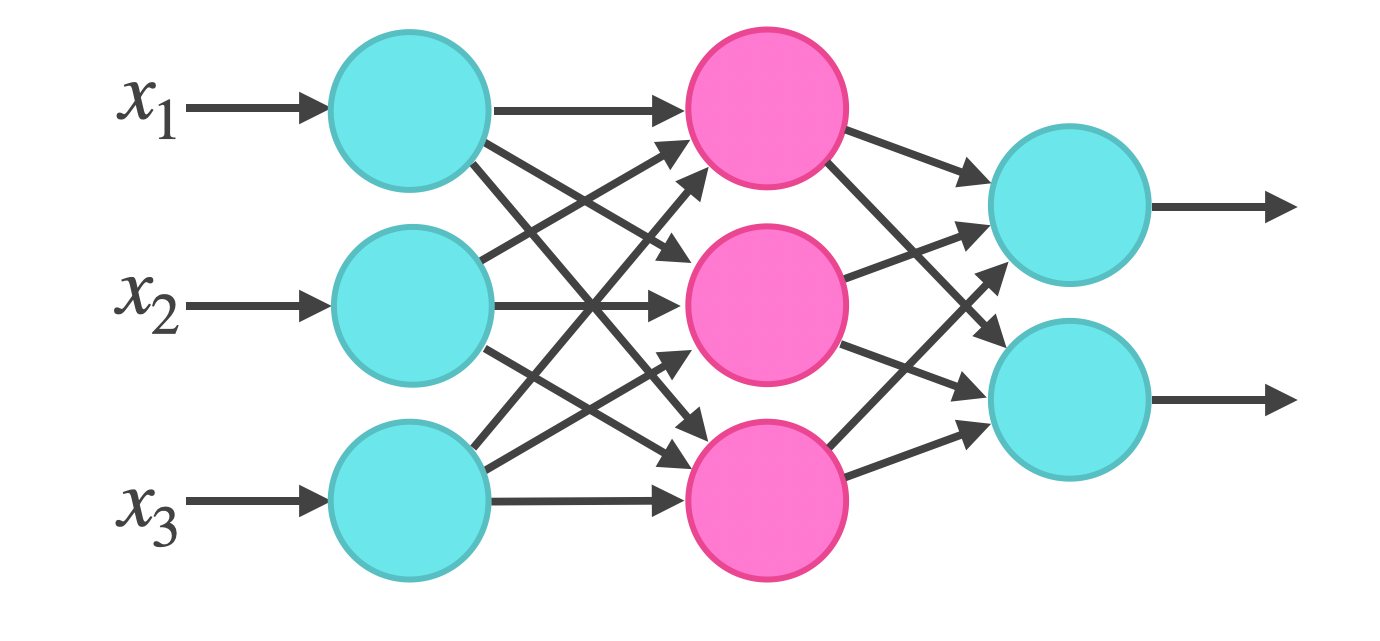
\includegraphics[width=0.65\textwidth]{Immagini/Generiche/esempioAplicativo_MPL.png}
    \caption{Esempio di un MLP.}
    
    %Figura 2.1: Esempio schematico di un neurone
\end{figure}

Come si osserva dalla figura, la rete è costituita dai seguenti elementi:

\begin{itemize}
    \item 3 neuroni in input (\(x_1, x_2, x_3\));
    \item Un livello nascosto (\(l=1\)) con 3 neuroni (\(h_1^{(1)}, h_2^{(1)}, h_3^{(1)}\));
    \item Un livello di output (\(l=2\)) con 2 neuroni (\({y}_1, {y}_2\)).
\end{itemize}

Definiamo i parametri della rete come segue:
\begin{itemize}
    \item Vettore di input: 
    \[\mathbf{X} = \begin{bmatrix} x_1 \\ x_2 \\ x_3 \end{bmatrix} =\begin{bmatrix} 1 \\ -2 \\ 0.5 \end{bmatrix}\]


    \item Matrici dei pesi: 
    \begin{multicols}{2}
        {
            \[
                \mathbf{W}^{(1)} = 
                \begin{bmatrix}
                    0.2 & -0.4 & 0.1 \\
                    -0.1 & 0.3 & -0.5 \\
                    0.7 & 0.2 & -0.3
                \end{bmatrix}
            \]
        }
        {
            \[
                \mathbf{W}^{(2)} = 
                \begin{bmatrix}
                    0.5 & -0.6 & 0.2 \\
                    -0.3 & 0.8 & -0.7
                \end{bmatrix}
            \]
        }
    \end{multicols}
    
    \item Vettori dei bias: 
    \begin{multicols}{2}
        {\[\mathbf{b}^{(1)} = \begin{bmatrix} 0.1 \\ -0.2 \\ 0.3 \end{bmatrix}\]}
        {\[\mathbf{b}^{(2)} = \begin{bmatrix} -0.1 \\ 0.4 \end{bmatrix}\]}
    \end{multicols}

    
    \item Come funzione di attivazione per $\sigma^{(1)}$ e per $\sigma^{(2)}$, utilizzeremo la funzione di \textbf{Heaviside} 
    con $\theta = 0$, definita nel seguente modo:
    \[
        \sigma(z) = 
        \begin{cases} 
        1 & \text{se } z \geq \theta, \\
        0 & \text{se } z < \theta.
        \end{cases}
    \]
\end{itemize}

\newpage
Ora passiamo a calcolare l'output della rete.
Utilizzando le formule \ref{MPL_LAYER} e \ref{MPL_OUTPUT}, l'output della rete 
può essere descritto come:

\[
    {\mathbf{y}} = \sigma^{(2)}\left( \mathbf{W}^{(2)}\left(\sigma^{(1)}\left( \mathbf{W}^{(1)}\mathbf{X} + {\mathbf{b}}^{(1)}\right)  \right)+ {\mathbf{b}}^{(2)}\right)
\]
\\
Iniziamo calcolando il prodotto matriciale \(\mathbf{W}^{(1)}\mathbf{X}\):

\[
\mathbf{W}^{(1)} \mathbf{X} = 
\begin{bmatrix}
0.2 & -0.4 & 0.1 \\
-0.1 & 0.3 & -0.5 \\
0.7 & 0.2 & -0.3
\end{bmatrix}
\begin{bmatrix}
1 \\ -2 \\ 0.5
\end{bmatrix}
=
\begin{bmatrix}
0.2(1) + (-0.4)(-2) + 0.1(0.5) \\
-0.1(1) + 0.3(-2) + (-0.5)(0.5) \\
0.7(1) + 0.2(-2) + (-0.3)(0.5)
\end{bmatrix}
=
\]
\[
= 
\begin{bmatrix}
0.2 + 0.8 + 0.05 \\
-0.1 - 0.6 - 0.25 \\
0.7 - 0.4 - 0.15
\end{bmatrix}
=
\begin{bmatrix}
1.05 \\ -0.95 \\ 0.15
\end{bmatrix}
\]
Ora sommiamo il bias:

\[
\mathbf{W}^{(1)} \mathbf{X} + \mathbf{b}^{(1)} = 
\begin{bmatrix}
1.05 \\ -0.95 \\ 0.15
\end{bmatrix}
+
\begin{bmatrix}
0.1 \\ -0.2 \\ 0.3
\end{bmatrix}
=
\begin{bmatrix}
1.15 \\ -1.15 \\ 0.45
\end{bmatrix}
\]

Infine, applichiamo la funzione di Heaviside (con \(\theta = 0\)) in modo
da ottenere il risultato del layer 1 ($\mathbf{h}^{(1)}$):

\[
\mathbf{h}^{(1)} =
\sigma^{(1)}\left( \mathbf{W}^{(1)} \mathbf{X} + \mathbf{b}^{(1)} \right) =
\begin{bmatrix}
\sigma(1.15) \\
\sigma(-1.15) \\
\sigma(0.45)
\end{bmatrix}
=
\begin{bmatrix}
1 \\
0 \\
1
\end{bmatrix}
\]


Ora calcoliamo il prodotto \(\mathbf{W}^{(2)} \mathbf{h}^{(1)}\):

\[
\mathbf{W}^{(2)} \mathbf{h}^{(1)} = 
\begin{bmatrix}
0.5 & -0.6 & 0.2 \\
-0.3 & 0.8 & -0.7
\end{bmatrix}
\begin{bmatrix}
1 \\ 0 \\ 1
\end{bmatrix}
=
\begin{bmatrix}
0.5(1) + (-0.6)(0) + 0.2(1) \\
-0.3(1) + 0.8(0) + (-0.7)(1)
\end{bmatrix}
=
\]
\[
= 
\begin{bmatrix}
0.5 + 0 + 0.2 \\
-0.3 + 0 - 0.7
\end{bmatrix}
=
\begin{bmatrix}
0.7 \\ -1.0
\end{bmatrix}
\]

Ora sommiamo il bias:

\[
\mathbf{W}^{(2)} \mathbf{h}^{(1)} + \mathbf{b}^{(2)} = 
\begin{bmatrix}
0.7 \\ -1.0
\end{bmatrix}
+
\begin{bmatrix}
-0.1 \\ 0.4
\end{bmatrix}
=
\begin{bmatrix}
0.6 \\ -0.6
\end{bmatrix}
\]

Infine, applichiamo la funzione di Heaviside al livello di output
in modo da ottenere il risultato del layer 2 (($\mathbf{h}^{(2)}$)):

\[
\mathbf{h}^{(2)}=
\sigma^{(2)}\left( \mathbf{W}^{(2)} \mathbf{h}^{(1)} + \mathbf{b}^{(2)} \right) =
\begin{bmatrix}
\sigma(0.6) \\
\sigma(-0.6)
\end{bmatrix}
=
\begin{bmatrix}
1 \\
0
\end{bmatrix}
\]

L'output finale della rete sara così:

\[
{\mathbf{y}} = \mathbf{h}^{(2)}= \begin{bmatrix} 1 \\ 0 \end{bmatrix}
\]


\section{Il Gradient Descent}

Per valutare quanto bene abbia "imparato" il modello si utilizza una 
\textit{loss function} (funzione di perdita) \( C \), talvolta indicata anche come 
\textit{cost function} (funzione di costo). 
Essa rappresenta una misura dell’errore del modello in termini di capacità di 
stimare la relazione tra un input \( x \) e il corrispondente output \( y \).

%\hspace{0.125cm}
La scelta della loss function da utilizzare dipende dal tipo di problema per 
cui è stato progettato il modello di rete neurale: per problemi di regressione, 
la loss function comunemente usata è il Mean Squared Error (MSE), ma ne esistono molte altre per specifiche
esigenze. La funzione di costo MSE è così definita:

\[
C(w, b) = \frac{1}{2n} \sum_{i=1}^n \|y(x) - a\|^2 = \frac{1}{2n} \sum_{i=1}^{n} \|y_i - \hat{y}_i\|^2
\]

dove \( w \) e \( b \) sono i vettori contenenti, rispettivamente, tutti i pesi e 
i bias della rete, \( x \) è il vettore degli elementi in input avente 
output \( y \), \( n \) è il numero totale di elementi del dataset e \( a \) è 
l’output di \( x \) stimato dalla rete.

Al fine di condurre il modello ad apprendere correttamente i dati presenti 
all’interno del training set, è necessario minimizzare la funzione \( C \): per 
farlo si utilizza l’algoritmo \textbf{Gradient Descent} (discesa del gradiente) 
\cite{GradientDescent_NeuralNetworks,GradientDescent_TowardsDataScience,GradientDescent_Medium}. 

\subsection{Cenni alle derivate parziali}
Prima di addentrasi a comprendere come funziona il Gradient Descent, accenniamo il 
funzionamento delle derivate parziali. In quanto vengono largamente 
utilizzate sia nel Gradient Descent che nella backpropagation.
In breve, una derivata parziale si utilizza sulle funzioni che hanno più variabili, 
come $f(x,y,z)$, e consiste nel calcolare la derivata della funzione rispetto a una 
singola variabile, considerando tutte le altri variabili come costanti.
Per indicare una derivata parziale di una $f$ rispetto a una generica variabile $x$, 
si utilizza la notazione $\frac{\partial f}{\partial x}$. 
Oppure può anche essere indicato la notazione $\partial_xf$ \cite{Derivate_parziali}.
Per capire il funzionamento, prendiamo una funzione di due variabili, ad 
esempio $f(x, y) = x^2 + 3xy + y^2$. 
La derivata parziale di $f$ rispetto a $x$ sarà: 
\[\frac{\partial f}{\partial x} = 2x + 3y\] 

Analogamente, la derivata parziale di $f$ rispetto a $y$ sarà: 
\[\frac{\partial f}{\partial y} = 3x + 2y\]

\subsection{Funzionamento del Gradient Descent}
Per comprendere meglio l’idea alla base del gradient descent, 
supponiamo inizialmente che $C$ sia una funzione di due variabili 
$v_1$ e $v_2$, ovvero $C(v_1, v_2)$. La variazione ($\Delta$) di ciascuna delle due componenti 
provocherà una variazione di $C$ esprimibile come:
\begin{equation}
    \Delta C \approx \frac{\partial C}{\partial v_1} \Delta v_1 + \frac{\partial C}{\partial v_2} \Delta v_2
    \label{eq:gd1}
\end{equation}

In cui:
\begin{itemize}
    \item $\frac{\partial C}{\partial v_1} \Delta v_1$: misura il contributo al cambiamento 
    totale $\Delta C$ dovuto ad una variazione di $v_1$ per il tasso di variazione di $C$ rispetto a $v_1$,  
    ovvero quanto velocemente varia $\Delta C$ spostandosi lungo l'asse $v_1$ mantenendo $v_2$ costate.
 

    \item $\frac{\partial C}{\partial v_2} \Delta v_2$: misura il contributo al cambiamento 
    totale $\Delta C$ dovuto ad una variazione di $v_2$ per il tasso di variazione di $C$ rispetto a $v_2$,  
    ovvero quanto velocemente varia $\Delta C$ spostandosi lungo l'asse $v_2$ mantenendo $v_1$ costate.
    
\end{itemize}

Per minimizzare $C$, è necessario trovare $\Delta v_1$ e $\Delta v_2$ tale che 
$\Delta C$ sia negativo. 

\begin{figure}[H]
    \centering
    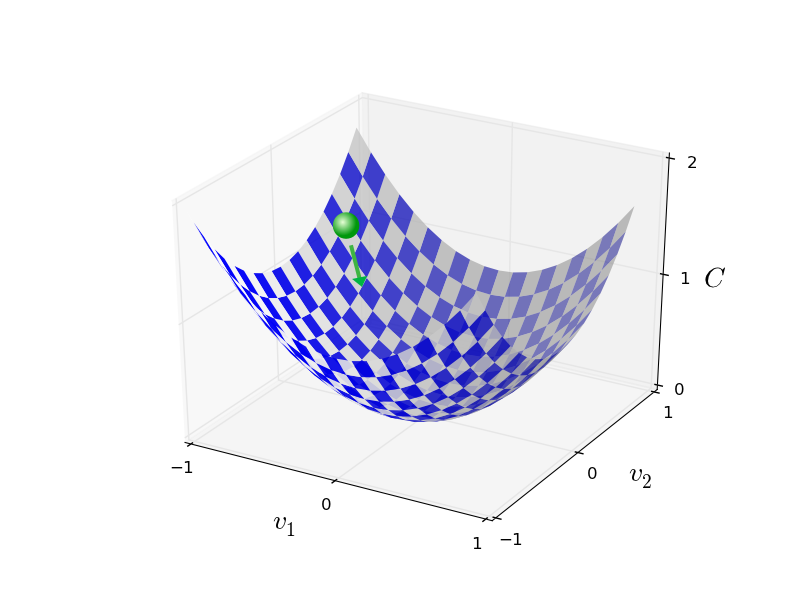
\includegraphics[width=0.8\textwidth]{Immagini/Grafici/valley_with_ball.png}
    \caption{Minimizzare la funzione $C$}

    %Figura 2.1: Esempio schematico di un neurone
\end{figure}

Definiamo il gradiente di $C$ come il vettore delle 
sue derivate parziali:
\begin{equation}
    \nabla C \equiv \left(
    \frac{\partial C}{\partial v_1},  
    \frac{\partial C}{\partial v_2}
    \right)^T
    \label{eq:gd2}
\end{equation}

e, ponendo $\Delta v = (\Delta v_1, \Delta v_2)^T$, è possibile riscrivere 
l’equazione \eqref{eq:gd1} come:
\begin{equation}
    \Delta C \approx \nabla C \cdot \Delta v
    \label{eq:gd3}
\end{equation}

L’importanza dell’equazione \eqref{eq:gd3} sta nel fatto che, affinché $C$ 
possa decrescere, è necessario scegliere $\Delta v$ in modo 
che $\Delta C$ sia negativo. In particolare, poniamo:
\begin{equation}
    \Delta v = -\eta \nabla C
\end{equation}
dove $\eta$ è un numero positivo comunemente noto come \textit{learning rate}, tipicamente avente 
un valore tra $1$ e $0$. 
Pertanto, l’equazione \eqref{eq:gd3} può essere riscritta come:
\begin{equation}
    \Delta C \approx -\eta \|\nabla C\|^2
\end{equation}

Poiché $\|\nabla C\|^2 \geq 0$, si ha la certezza che $\Delta C \leq 0$. Questa procedura permetterà di aggiornare le componenti di $v$ che saranno uguali a:
\begin{equation}
    v \to v' = v - \eta \nabla C
\end{equation}

Nel nostro caso, il vettore \textbf{$v$} è sostituito da $w$ e $b$, ovvero i 
vettori di pesi e bias. Parleremo di epoca di training quando ciascun elemento 
del dataset verrà processato sia in avanti (\textit{forward}) sia all’indietro 
(\textit{backward}) dalla rete una sola volta.

Per ogni epoca, una volta calcolata la loss function $C$, è necessario dunque 
derivare $C$ rispetto a $w$ e rispetto a $b$. Al termine di ogni epoca verranno 
infine aggiornati i valori di \textbf{$w$} e di \textbf{$b$} nel seguente modo:
\begin{equation}
    w_i \to w_i' = w_i - \eta \frac{\partial C}{\partial w_i} \quad \forall i = 1, \dots, n
    \label{eq:aggiornamentoPesi}
\end{equation}
\begin{equation}
    b_i \to b_i' = b_i - \eta \frac{\partial C}{\partial b_i} \quad \forall i = 1, \dots, n
    \label{eq:aggiornamentoBias}
\end{equation}


Il \textit{learning rate} $\eta$ regolerà l’aggiornamento di $w$ e $b$: più 
grande sarà $\eta$, più velocemente l’algoritmo tenderà a convergere verso il 
punto che minimizza $C$.
Tuttavia, un learning rate elevato può condurre a degli eccessivi "salti" all’interno della
funzione, il che potrebbe causare una mancanza di convergenza.
Viceversa, la scelta di un learning rate eccessivamente piccolo potrebbe rallentare 
parecchio il processo di convergenza, rendendo necessario un numero di epoche più elevato
al fine di raggiungere risultati accettabili.

\begin{figure}[H]
    \centering
    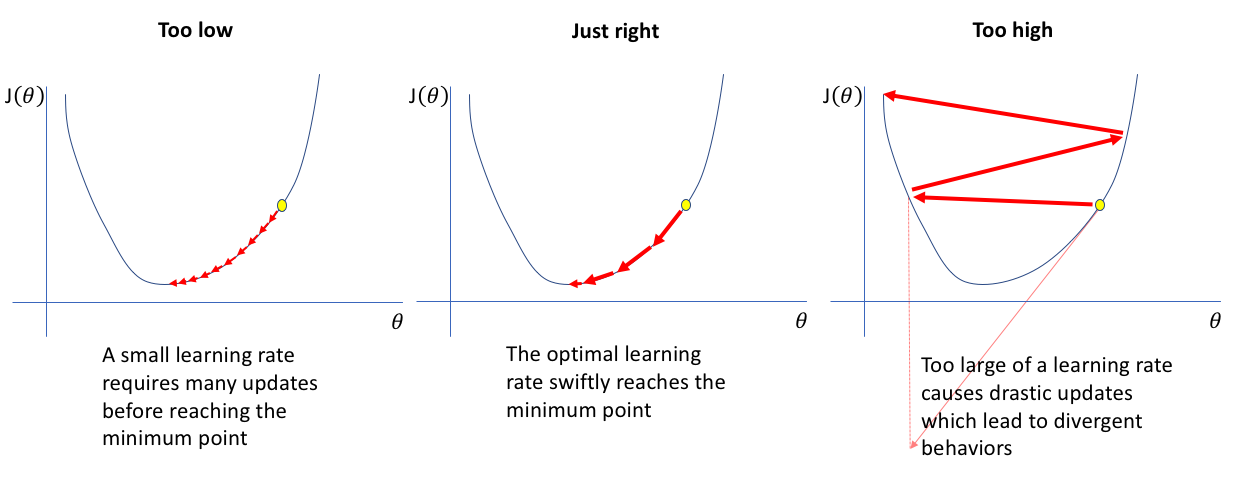
\includegraphics[width=1\textwidth]{Immagini/Grafici/esempioLR.png}
    \caption{ I grafici mostrano il differente processo di convergenza verso il punto di minimo
    globale di $C$ \cite{LearningRate_optimizer}}.

    %Figura 2.1: Esempio schematico di un neurone
\end{figure}

\'E possibile applicare l’algoritmo del gradient descent calcolando il gradiente 
sull'intero dataset oppure selezionare uno o più elementi ad ogni 
iterazione: questo viene indicato con il termine \textbf{batch}, ovvero il numero totale di 
campioni del dataset utilizzati per calcolare il gradiente in una singola 
operazione. La scelta di un opportuno gruppo di elementi del
dataset influisce sull'aggiornamento di $w$ e $b$, pertanto influisce anche sul processo di 
convergenza della \textit{loss function}.
Poiché l’algoritmo del gradient descent è una procedura iterativa, 
risulta abbastanza evidente che effettuare il training di un modello per una singola 
epoca comporterà un solo aggiornamento di pesi e bias. Viceversa, un numero 
eccessivo di epoche di training può condurre il modello ad adattarsi eccessivamente 
ai dati di training e, di conseguenza, andare incontro al problema 
dell’\textit{overfitting}, ovvero l'incapacità di generalizzare i dati.

\section{Ottimizzatori}
Gli ottimizzatori sono delle tecniche che vengono utilizzate per migliorare il processo 
di addestramento di una rete neurale \cite{ALL_DEEP_LEARNING,LearningRate_optimizer}.

\subsection{Full Batch Gradient Descent}
Il \textit{full batch gradient descent} \cite{GradientDescent_NeuralNetworks, LearningRate_optimizer} calcola la loss function considerando, ad ogni iterazione,
tutti gli elementi presenti all’interno del dataset: $C$ sarà dunque la 
loss function media calcolata sull'intero dataset, 
ovvero $C = \frac{1}{n}\sum_{i}^{}C_i$. La procedura di aggiornamento di $w$
e $b$ è la medesima descritta dalle equazioni \eqref{eq:aggiornamentoPesi} e \eqref{eq:aggiornamentoBias}. 
Nonostante la semplicità
a livello intuitivo della procedura, essa comporta diversi svantaggi: poiché vengono
utilizzati tutti gli elementi presenti all’interno del dataset ad ogni singola iterazione, tale
operazione risulta essere parecchio onerosa in presenza di dataset di grandi dimensioni.
Un altro problema consiste nella sua scarsa dinamicità: per migliorare il modello con
nuovi dati è necessario ripetere il processo di training sull'intero dataset.
Inoltre, tale procedura risulta essere molto soggetta al problema dei minimi locali.

\subsection{Stochastic Gradient Descent}

Uno dei problemi del \textit{full batch gradient descent} \cite{GradientDescent_NeuralNetworks, LearningRate_optimizer} riguardava la necessità di 
calcolare $\nabla C$
su tutti gli elementi del dataset, a prescindere dalla dimensione di esso.
L’approccio dello stochastic gradient descent è differente: $\nabla C$ non è più la media sui
$\nabla C$ calcolati sull'intero dataset, bensì viene stimato da un singolo elemento del dataset
scelto in maniera casuale.
A differenza del precedente approccio, la scelta di un singolo elemento del dataset per
il calcolo di $C$ porta ad un notevole miglioramento in termini di tempo d’esecuzione
dell’algoritmo. Da un punto di vista grafico, è possibile che $C$ tenda parecchio ad
oscillare: tali oscillazioni potrebbero condurre la loss function ad uscire più facilmente
da punti di minimo locale.

\subsection{Mini Batch Gradient Descent}
Lo stochastic gradient descent riesce tuttavia a risolvere solo parzialmente il 
problema dei minimi locali.
Una via di mezzo tra le tecniche precedentemente descritte è il \textit{mini batch 
gradient descent}\cite{GradientDescent_NeuralNetworks, LearningRate_optimizer}: all’interno del dataset, ad ogni epoca viene estratto un 
sottoinsieme di elementi casuali del dataset e la loss function calcolata è la media 
delle loss functions calcolate all’interno del sottoinsieme. Pertanto, scelto 
un numero $m < n$ come batch size, $\nabla C$ sarà uguale a:

\begin{equation}
    \nabla C = \frac{1}{n}\sum_{i} \nabla C_i \approx \frac{1}{m}\sum_{j=1}^{m} \nabla C_j
\end{equation}

e le equazioni \eqref{eq:aggiornamentoPesi} e \eqref{eq:aggiornamentoBias} 
diventeranno:

\begin{equation}
    w_i \to w_i' = w_i - \frac{\eta}{m} \cdot \sum_{j}^{m} \frac{\partial C_{X_j}}{\partial w_i} %\quad \forall i = 1, \dots, n
\end{equation}
\begin{equation}
    b_i \to b_i' = b_i - \frac{\eta}{m} \cdot \sum_{j}^{m} \frac{\partial C_{X_j}}{\partial b_i} %\quad \forall i = 1, \dots, n
\end{equation}

dove le somme sono su tutti gli esempi di addestramento $X_j$ presenti nel mini-batch corrente.
Finito il processo di aggiornamento dei parametri, si seleziona un altro mini-batch e si 
ripete l'operazione finché non abbiamo esaurito gli input di addestramento. 
A quel punto ricominciamo con una nuova epoca di addestramento.

\subsection{Full Batch vs Stochastic vs Mini Batch}
All’interno della figura \ref{fig:paragonebatch} è rappresentato il confronto tra le traiettorie prodotte 
dalle tre tecniche citate. Si può osservare come lo stochastic gradient descent e il mini 
batch gradient descent producano traiettorie che tendono ad andare "a zig-zag". Questo 
comportamento è dovuto al fatto che, rispettivamente, vengono scelti un elemento ed 
un sottocampione dal dataset di partenza. Pertanto, a differenza del full batch gradient 
descent, non stiamo calcolando il gradiente di $C$, bensì una sua approssimazione.

 \begin{figure}[H]
    \centering
    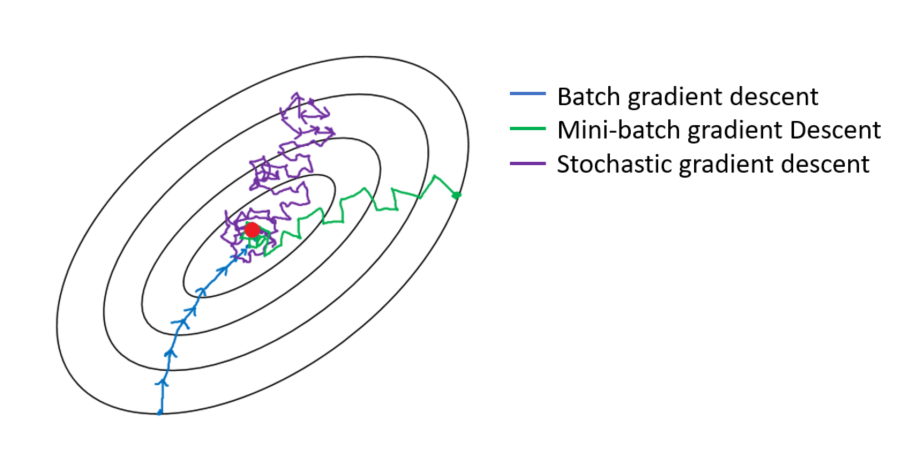
\includegraphics[width=0.8\textwidth]{Immagini/Grafici/paragonebatch.png}
    \caption{Confronto tra le traiettorie prodotte dagli algoritmi basati sul gradient descent \cite{Full Batch vs Stochastic vs Mini Batch}.}
    \label{fig:paragonebatch}
    %Figura 2.1: Esempio schematico di un neurone
\end{figure}

Queste sono soltanto alcune delle tante strategie di ottimizzazione 
che si possono utilizzare per migliorare l'apprendimento del modello.


\section{L'algoritmo della Backpropagation}
Come accennato precedentemente, l'algoritmo della Backpropagation ha portato 
grandi progressi nell'implementazione delle reti neurali.
L’algoritmo si basa sulla modifica sistematica dei 
pesi delle connessioni tra neuroni cosicché l’output della rete coincida 
sempre di più con il risultato atteso 
\cite{GradientDescent_NeuralNetworks,ALL_DEEP_LEARNING,ASPETTI_MLP_1,ASPETTI_MLP_2,Introduzione_backpropagation}.
Questo algoritmo è costituito da due fasi principali:

\begin{itemize}
    \item \textbf{Forward propagation}: Il processo del calcolo delle predizioni che parte dai 
    coefficienti per poi terminare con l’errore rispetto al risultato atteso.
    \item \textbf{backward propagation}: il processo che permette di ottimizzare i 
    coefficienti $w$ e $b$ partendo dal l’errore calcolato precedentemente.
\end{itemize}

Questo processo, introdotto già nel 1970, acquisì notevole importanza
nel 1986, anno in cui D. Rumelhart, G. Hinton e R. Williams evidenziarono quanto una 
rete neurale apprenda più velocemente grazie alla backpropagation rispetto alle
tecniche utilizzate in precedenza. Ancora oggi, esso assume un’importanza notevole al fine 
dell’apprendimento delle più moderne reti neurali profonde \cite{Articolo_backpropagation}.

\subsection{Il prodotto di Hadamard}
L'algoritmo di backpropagation si basa su comuni operazioni algebriche lineari, 
come l'addizione di vettori, la moltiplicazione di un vettore per una matrice e così via. 
La backpropagation si basa anche sul prodotto di Hadamard \cite{prodotto_Hadamard}, 
un'operazione matematica non 
comunemente utilizzata.
In particolare, supponiamo di avere due matrici, $A$ e $B$, l'operazione del prodotto di Hadamard
tra le due matrici, denotata con $A \odot B$, è definita nel seguente modo:
\begin{equation}
    (A \odot B)_{ij} = A_{ij} \cdot B_{ij}, \quad \forall i,j
\end{equation}

In pratica consiste in un'operazione di prodotto elementare tra gli elementi di ogni matrice. 
Pertanto è anche importante che le due matrici abbiano la medesima dimensione.
Ad esempio, consideriamo queste due matrici:
\[
A = \begin{bmatrix}
1 & 2 & 3 \\
4 & 5 & 6 \\
7 & 8 & 9
\end{bmatrix}, \cdot
B = \begin{bmatrix}
9 & 8 & 7 \\
6 & 5 & 4 \\
3 & 2 & 1
\end{bmatrix}.
\]

Il prodotto di Hadamard \( A \odot B \) è calcolato come:
\[
A \odot B = \begin{bmatrix}
1 \cdot 9 & 2 \cdot 8 & 3 \cdot 7 \\
4 \cdot 6 & 5 \cdot 5 & 6 \cdot 4 \\
7 \cdot 3 & 8 \cdot 2 & 9 \cdot 1
\end{bmatrix}
= \begin{bmatrix}
9 & 16 & 21 \\
24 & 25 & 24 \\
21 & 16 & 9
\end{bmatrix}.
\]

\subsection{Funzionamento della Backpropagation}
La backpropagation consiste nel comprendere come la modifica dei pesi e dei bias in una rete 
modifichi la funzione di costo. 
Ciò significa calcolare le derivate parziali $\frac{\partial C}{\partial w^{(l)}_{jk}}$ e 
$\frac{\partial C}{\partial b^{(l)}_{j}}$. Ma per calcolarli, introduciamo prima una quantità 
intermedia, $\delta_{j}^{(l)}$, ovvero l’errore presente nel neurone $j$-esimo del layer $l$-esimo
layer, $z_{j}^{(l)}$.
L’aggiunta di tale termine di errore al neurone $z_{j}^{(l)}$ porterà alla modifica 
della funzione di attivazione associata 
ad esso, la quale sarà adesso uguale a $\sigma (z_{j}^{(l)} + \Delta_{j}^{(l)})$
propagandosi all’interno della
 rete e causando così un’altrettanto modifica alla loss function totale, la quale subirà
 una variazione di $\frac{\partial C}{\partial z_{j}^{(l)}}\Delta z_{j}^{(l)}$.

 E’ possibile dunque monitorare la variazione della loss function facendo variare il
 termine di errore  $\delta_{j}^{(l)}$, definito come

 \begin{equation}
    \delta_{j}^{(l)} = \frac{\partial C}{\partial z_{j}^{(l)}}
 \end{equation}

 La backpropagation si basa principalmente su quattro equazioni, le quali costituiscono
 la base per il calcolo del gradiente di $C$ e del termine di errore $\delta$:

 \begin{itemize}
    \item  Equazione per l’errore all’interno dell'layer di output:
    \begin{equation}
        \delta_{j}^{(L)} = \frac{\partial C}{\partial a_{j}^{(L)}}\sigma ' (z_{j}^{(L)}) 
        \label{eq:backpropagation1}
    \end{equation}
    Dove il primo termine $\frac{\partial C}{\partial a_{j}^{(L)}}$ misura la velocità con cui il 
    costo cambia in funzione del j-esimo output di attivazione. Mentre il secondo termine 
    $\sigma ' (z_{j}^{(L)}) $ (dove $\sigma'$ è la derivata della funzione di attivazione $\sigma$)
    misura la velocità con cui la funzione di attivazione $\sigma$ cambia in $z_{j}^{(L)}$.
    Nella forma matriciale l'equazione \eqref{eq:backpropagation1} diventa:
    \begin{equation}
        \delta^{(L)} = \nabla_{a}C \odot \sigma '(z^{(L)}) 
    \end{equation}

    \item Equazione per l’errore $\delta^{(l)}$ espresso come errore del layer successivo:
    \begin{equation}
        \delta^{(l)} = ((W^{(l+1)})^{T} \delta^{(l+1)}) \odot \sigma '(z^{(L)})
        \label{eq:backpropagation2}
    \end{equation}
    Dove $(W^{(l+1)})^{T}$ è la trasposta della matrice dei pesi $W^{(l+1)}$ per il $(l+1)$-esimo layer. 
    Questa equazione sembra complicata, ma ogni elemento ha una precisa interpretazione. 
    Supponiamo di conoscere l'errore $\delta^{(l+1)}$. Quando applichiamo la matrice dei pesi 
    trasposta, $(W^{(l+1)})^{T}$, possiamo pensare intuitivamente a questo come allo spostamento 
    dell'errore all'indietro attraverso la rete, dandoci una sorta di misura dell'errore 
    all'output dell'$l$-esimo layer. Quindi svolgiamo il prodotto di Hadamard $\odot$ con 
    $\sigma '(z_{j}^{(l)})$. Questo sposta l'errore all'indietro attraverso la funzione di 
    attivazione del layer $l$, dandoci l'errore $\delta^{(l)}$ nell'input ponderato allo strato $l$.

    \item  Equazione per la variazione della loss function rispetto a qualsiasi bias:
    \begin{equation}
        \frac{\partial C}{\partial b_{j}^{(l)}} = \delta_{j}^{(l)}
        \label{eq:backpropagation3}
    \end{equation}

    \item Equazione per la variazione della loss function rispetto a qualsiasi peso:

    \begin{equation}
        \frac{\partial C}{w_{jk}^{(l)}} = a_{k}^{(l-1)}\delta_{j}^{(l)}
        \label{eq:backpropagation4a}
    \end{equation}

    L'equazione può essere riscritta in una notazione meno indicizzata come

    \begin{equation}
        \frac{\partial C}{w_{jk}^{(l)}} = a_{in}\delta_{out}
        \label{eq:backpropagation4b}
    \end{equation}

    dove si intende che $a_{in}$ è l'attivazione dell'input del neurone al peso $w$, e $\delta_{out}$
    è l'errore dell'output del neurone dal peso $w$. Ingrandendo per guardare solo il peso $w$, 
    e i due neuroni collegati da quel peso, possiamo rappresentarlo come:

    \begin{figure}[H]
        \centering
        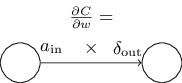
\includegraphics[width=0.25\textwidth]{Immagini/Generiche/tikz20.png}
        \caption{Rappresentazione dell'equazione \eqref{eq:backpropagation4b}.}
        %Figura 2.1: Esempio schematico di un neurone
    \end{figure}

\end{itemize}


Come si può intuire, combinando le equazioni \eqref{eq:backpropagation1} e \eqref{eq:backpropagation2}, possiamo computare l'errore
$\delta^{(l)}$ per ogni layer della rete, facendo propagare l'errore dall'output layer fino all'input 
layer.
Mentre le equazioni \eqref{eq:backpropagation1} e \eqref{eq:backpropagation1} mostrano le relazioni 
tra $\delta$ e le derivate parziali calcolate rispetto a $w$ e $b$.

\subsection{Applicazione della Backpropagation}

Nella pratica è bene combinare l’algoritmo di \textit{backpropagation} con un’algoritmo basato 
sul \textit{gradient descent}. Supponendo di utilizzare un mini batch gradient descent,
con batch size di $m < n$ elementi (dove $n$ è la dimensione del dataset), è possibile vedere come
l’azione combinata dei due algoritmi agisce sul processo di training 
\cite{GradientDescent_NeuralNetworks}:

\begin{enumerate}
    \item \textbf{Input}: Selezione casuale di $m$ valori di input all’interno del dataset
    \item \textbf{Feedforward}: $\forall x_i \in \{x_1, x_2, \dots, x_m\}$ e $\forall l \in
    \{2,3, \dots, L\}$ si \\ computa $z^{(l)} = W^{(l)}a^{(l-1)} +b^{(l)}, a^{(l)} = \sigma(z^{(l)})$
    
    \item \textbf{Output error}: Si calcola il vettore $\delta^{(L)} = \nabla_{a}C \odot \sigma '(z^{(L)})$ 
    \item \textbf{Backpropagate the error}: $\forall l \in \{L-1, L-2, \dots, 3, 2\}$ si calcola \\
    $\delta^{(l)} = ((W^{(l+1)})^{T} \delta^{(l+1)}) \odot \sigma '(z^{(L)})$

    \item \textbf{Gradient descent}: $\forall l \in \{L-1, L-2, \dots, 3, 2\}$ si esegue:
    \begin{itemize}
        \item aggiornamento di $w$ : 
        \begin{equation}
            w_i \to w_i' = w_i - \frac{\eta}{m} \cdot \sum_{x} (a^{(l-1)})^{T}\delta^{(l)} %\quad \forall i = 1, \dots, n
        \end{equation}
        \item aggiornamento di $b$ : 
        \begin{equation}
            b_i \to b_i' = b_i - \frac{\eta}{m} \cdot \sum_{x} \delta^{(l)} %\quad \forall i = 1, \dots, n
        \end{equation}
    \end{itemize}
\end{enumerate}


\section{Altre funzione di attivazione}
La scelta di un’opportuna funzione di attivazione assume un ruolo molto importante:
l’output restituito da una rete neurale è fortemente condizionato dalla funzione di
attivazione utilizzata, la quale possiede un ruolo molto importante anche nel processo
e nella velocità di convergenza della rete neurale e nella sua accuratezza.
Inoltre, nelle moderne reti neurali profonde, la scelta della funzione d’attivazione da
utilizzare dipende dal tipo di layer a cui essa è associata. Nel corso degli anni sono
state utilizzate diverse funzioni di attivazione: binarie, lineari e non lineari. Diamo
un’occhiata alle più comuni 
\cite{ActivationFunctions_NetAI,ALL_DEEP_LEARNING, ActivationFunctions_MEDIUM}:

\subsection{Funzione Sigmoide}
La funzione sigmoide è definita come segue:

\begin{multicols}{2}
    {
        \begin{figure}[H]
            \centering
            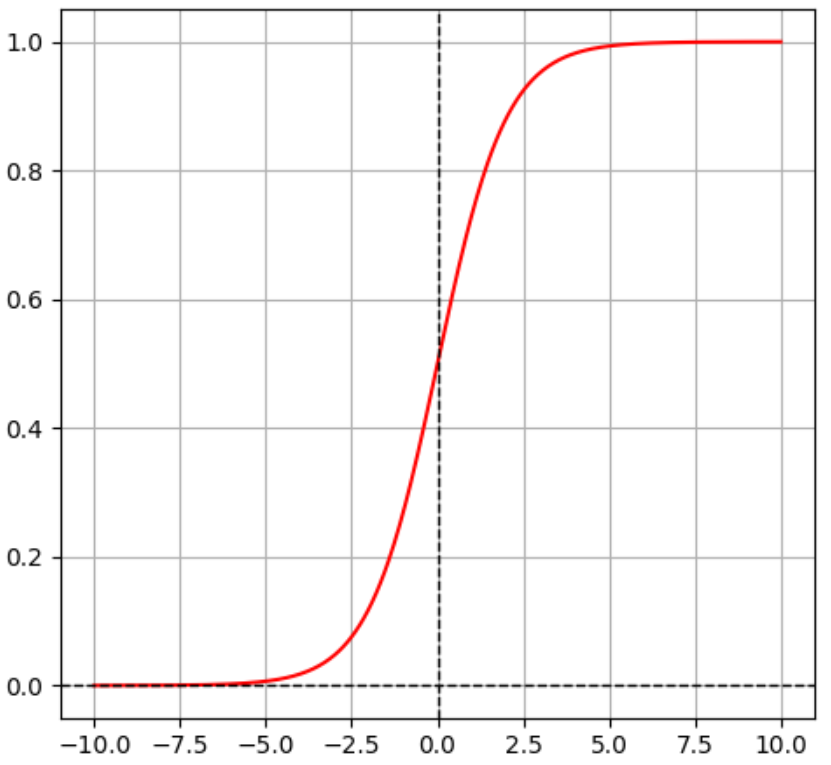
\includegraphics[width=0.40\textwidth]{Immagini/Grafici/graficoSigmoide.png}
            \caption{Grafico della sigmoide}
        \end{figure}
    }
    {
        \begin{itemize}
            \item \textbf{Equazione:}
            \begin{equation}
                \sigma(z) = \frac{1}{1 + e^{-z}}
            \end{equation}
                
            \item \textbf{Derivata:}
            \begin{equation}
                \frac{d}{dz}\sigma(z)  = \sigma(z) \cdot (1 - \sigma(z))
            \end{equation}
        \end{itemize}
    }
\end{multicols}

Poiché la funzione sigmoide restituisce in output un valore appartenente all’intervallo
 $[0, 1]$, essa viene utilizzata spesso come funzione di attivazione dell’output layer per
 modelli di classificazione ed il valore restituito in output assume un valore probabilistico
 se l’output è binario. Tuttavia, in problemi di classificazione multiclasse, 
 la sigmoide non è particolarmente adatta poiché manca di una normalizzazione 
 globale delle probabilità tra le varie classi.

Inoltre presenta delle limitazioni, come il problema del vanishing gradient, che
consiste nella progressiva riduzione del valore del gradiente man mano che si 
propaga all’indietro attraverso i livelli della rete neurale durante il 
processo di backpropagation.

Ciò comportava, se la rete presentava tanti layer interni con questa funzione di 
attivazione, il "congelamento" dell'apprendimento dei valori dei pesi durante 
la fase di training.



\subsection{Funzione Tanh (Tangente Iperbolica)}
Un’altra funzione di attivazione utilizzata è la funzione 
tangente iperbolica (tanh), la quale restituisce 
valori all’interno dell’intervallo $[-1, 1]$.
\begin{multicols}{2}
    {
        \begin{figure}[H]
            \centering
            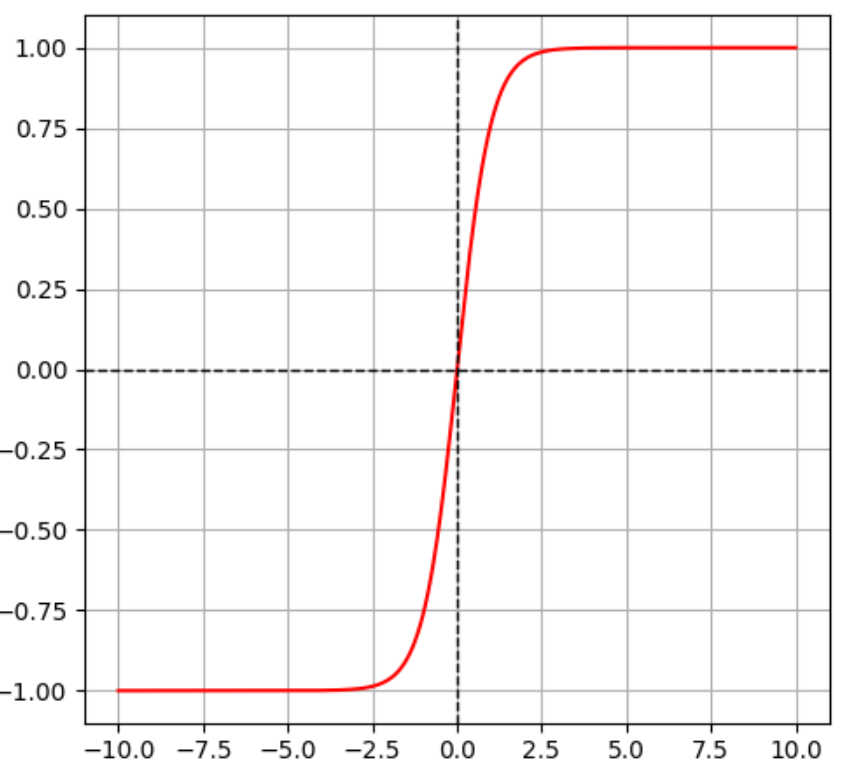
\includegraphics[width=0.40\textwidth]{Immagini/Grafici/graficoTanh.png}
            \caption{Grafico della Tanh}
        \end{figure}
    }
    {
        \begin{itemize}
            \item \textbf{Equazione:}
            \begin{equation}
                \sigma(z) = \tanh(z) = \frac{e^z - e^{-z}}{e^z + e^{-z}}
            \end{equation}
                
            \item \textbf{Derivata:}
            \begin{equation}
                \frac{d}{dz}\sigma(z)  = 1 - \sigma(z)^2
            \end{equation}
        \end{itemize}

        La funzione mappa l'input in un intervallo tra -1 e 1, 
        utile per normalizzare i dati. Anche questa funzione può 
        soffrire del vanishing gradient.
    }
\end{multicols}





\subsection{ReLU (Rectified Linear Unit)}
La funzione ReLU è così definita:
\begin{multicols}{2}
    {
        \begin{figure}[H]
            \centering
            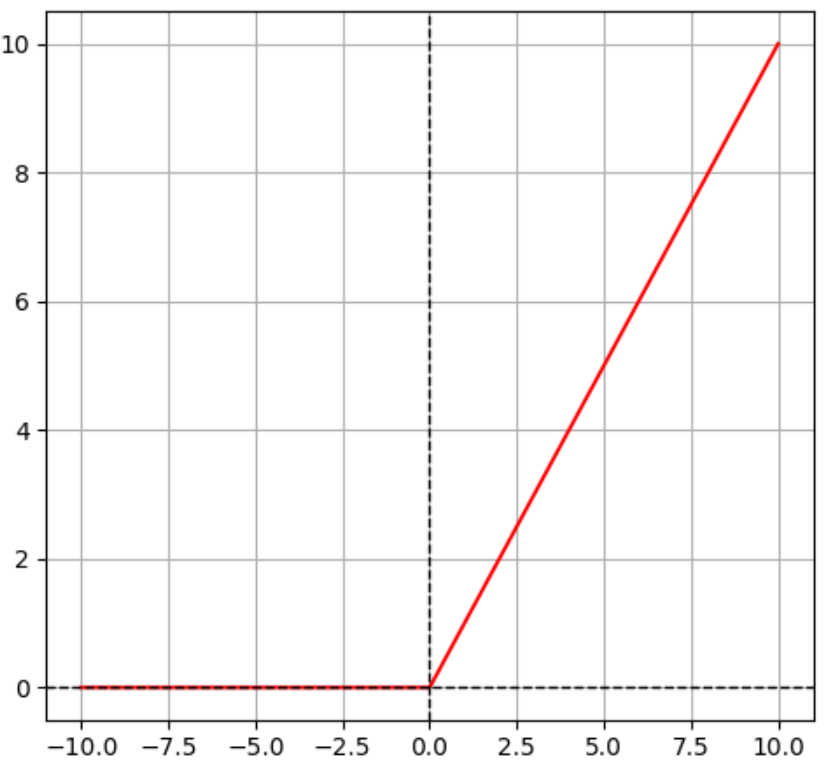
\includegraphics[width=0.40\textwidth]{Immagini/Grafici/graficoRelu.png}
            \caption{Grafico della Tanh}
        \end{figure}
    }
    {
        \begin{itemize}
            \item \textbf{Equazione:}
            \begin{equation}
                \sigma(z) = \max(0, z)
            \end{equation}
                
            \item \textbf{Derivata:}
            \begin{equation}
                \frac{d}{dz}\sigma(z) = \begin{cases}
                    1 & \text{se } z > 0, \\
                    0 & \text{se } z \leq 0.
                \end{cases}
            \end{equation}
        \end{itemize}
        Essa sarà quindi uguale a $z$ per $z > 0$, mentre sarà 
        nulla per tutti gli altri valori.
        \'E la funzione di attivazione maggiormente utilizzata 
        nelle reti neurali artificiali e ha sostituito nel corso 
        degli anni le funzioni tangente iperbolica e sigmoide.
    }
\end{multicols}


Il motivo principale è dovuto al fatto che la tanh e la sigmoide 
hanno una derivata prima molto piccola, la
quale tende velocemente a 0.
Poiché il training di una rete neurale si basa sulla discesa del gradiente, la 
moltiplicazione per un valore prossimo a 0 porta i layer più profondi della rete ad un apprendimento
 più lento. \'E inoltre molto facile da calcolare (da un punto di vista computazionale, è necessario
 solamente un confronto per determinarne l’output) e ciò si traduce, nel caso di reti
 neurali molto profonde, in un notevole risparmio in termini di costo computazionale





\subsection{Leaky ReLU}
La funzione Leaky ReLU è definita come:

\begin{multicols}{2}
    {
        \begin{figure}[H]
            \centering
            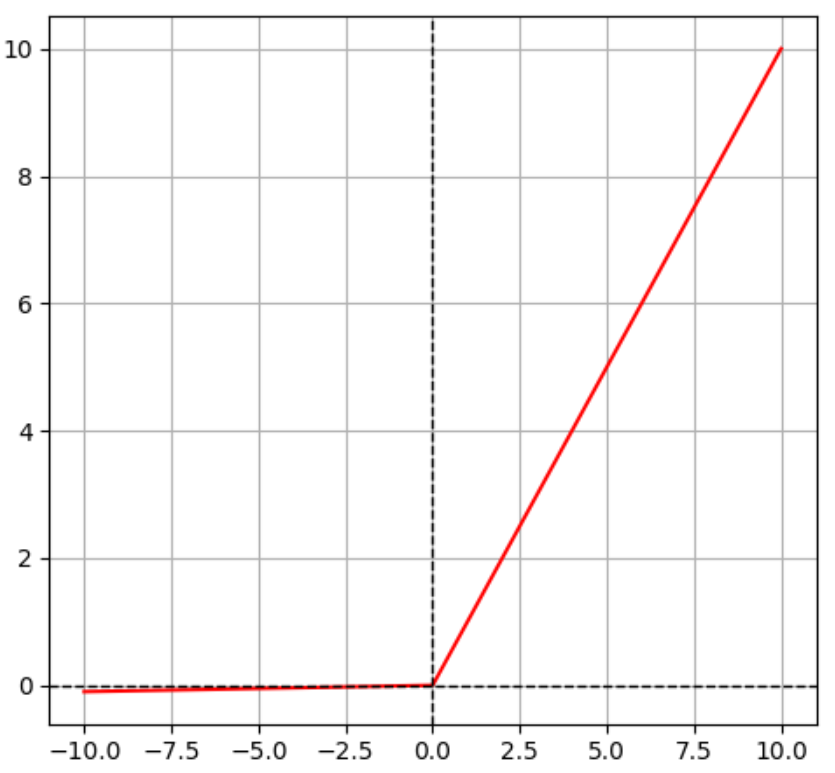
\includegraphics[width=0.40\textwidth]{Immagini/Grafici/graficoLeakyRelu.png}
            \caption{Grafico della Tanh}
        \end{figure}
    }
    {
        \begin{itemize}
            \item \textbf{Equazione:}
            \begin{equation}
                \sigma(z) = \begin{cases}
                    z & \text{se } z > 0, \\
                    \alpha z & \text{se } z \leq 0,
                \end{cases}
            \end{equation}
            dove \(\alpha > 0\) è un parametro fissato.
            \item \textbf{Derivata:}
            \begin{equation}
                \frac{d}{dz}\sigma(z) = \begin{cases}
                    1 & \text{se } z > 0, \\
                    \alpha & \text{se } z \leq 0.
                \end{cases}
            \end{equation}
        \end{itemize}
    }
\end{multicols}


Leaky relu è il miglioramento della funzione Relu. La funzione Relu può uccidere 
alcuni neuroni in ogni iterazione, questo è noto come condizione di relu morente. 
Leaky relu può superare questo problema, invece di dare 0 per valori negativi, 
utilizzerà una componente di input relativamente piccola per calcolare l’output, 
quindi non ucciderà mai alcun neurone.





\subsection{ELU (Exponential Linear Unit)}
La funzione ELU è definita come:
\begin{multicols}{2}
    {
        \begin{figure}[H]
            \centering
            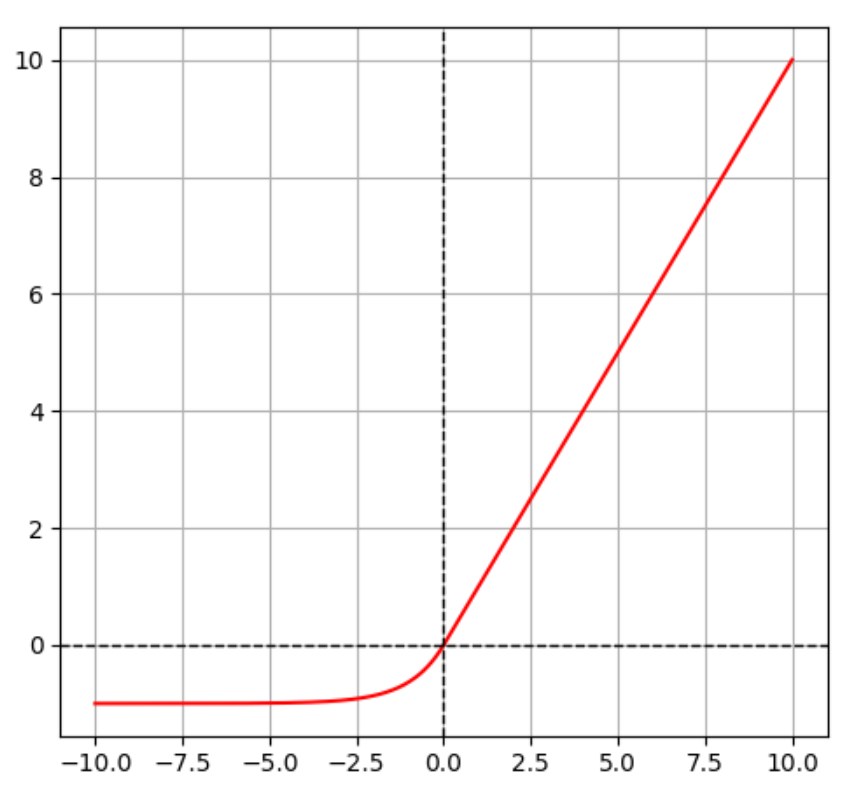
\includegraphics[width=0.40\textwidth]{Immagini/Grafici/graficoElu.png}
            \caption{Grafico della Tanh}
        \end{figure}
    }
    {
        \begin{itemize}
            \item \textbf{Equazione:}
            \begin{equation}
                \sigma(z) = \begin{cases}
                    z & \text{se } z > 0, \\
                    \alpha(e^z - 1) & \text{se } z \leq 0,
                \end{cases}
            \end{equation}
            dove \(\alpha > 0\) è un parametro fissato.
            \item \textbf{Derivata:}
            \begin{equation}
                \frac{d}{dz}\sigma(z) = \begin{cases}
                    1 & \text{se } z > 0, \\
                    \alpha e^z & \text{se } z \leq 0.
                \end{cases}
            \end{equation}
        \end{itemize}
    }
\end{multicols}

L'ELU è un’altra variazione di Relu che cerca di rendere le attivazioni più 
vicine allo zero che accelera l’apprendimento. Ha mostrato una migliore accuratezza 
della classificazione rispetto a Relu. Gli ELU hanno valori negativi che spingono la 
media delle attivazioni più vicino a zero.


\subsection{Swish}
La funzione Swish è così definita come:
\begin{multicols}{2}
    {
        \begin{figure}[H]
            \centering
            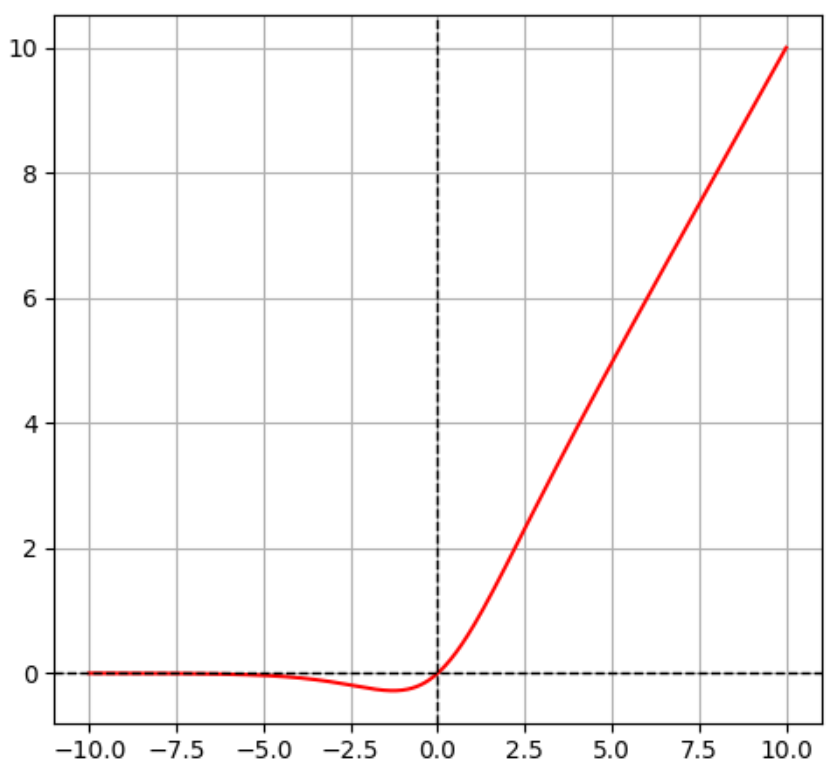
\includegraphics[width=0.40\textwidth]{Immagini/Grafici/graficoSwish.png}
            \caption{Grafico della Tanh}
        \end{figure}
    }
    {
        \begin{itemize}
            \item \textbf{Equazione:}
            \begin{equation}
                \sigma(z) = z \cdot \text{sigmoid}(z) = \frac{z}{1+e^{-z}}
            \end{equation}
            \item \textbf{Derivata:}
            \begin{equation}
                \frac{d}{dz}\sigma(z) = \sigma(z) + \text{sigmoid}(x) \cdot (1 - \sigma(z))
            \end{equation}
        \end{itemize}
    }
\end{multicols}

Questa funzione combina le proprietà della ReLU e della sigmoide, 
risultando spesso in migliori prestazioni.

La funzione Swish è stata proposta dal team Brain di Google. I loro esperimenti 
hanno dimostrano che la Swish tende a funzionare più velocemente della Relu in modelli 
profondi su diversi set di dati impegnativi.

\subsection{Softmax}
Per problemi di classificazione, la funzione di attivazione sigmoide si presta bene nel
caso in cui si hanno solamente due classi.
Qualora il numero di classi sia maggiore, si utilizza la funzione di attivazione softmax,
così definita \cite{ActivationFunctions_Softmax, ActivationFunctions_MEDIUM}:
\begin{equation}
    \sigma(z) = \frac{e^{z_i}}{\sum_{j=1}^K e^{z_j}}, \quad \text{per } i = 1, \dots, K
\end{equation}

Softmax è fondamentalmente una funzione vettoriale. Prende un vettore come input e 
produce un vettore come output. In altre parole, ha più ingressi e uscite.

La funzione di attivazione Softmax viene usata sempre nell'output layer, facendo
in modo che che l'output della rete assuma un’interpretazione probabilistica.

\begin{figure}[H]
    \centering
    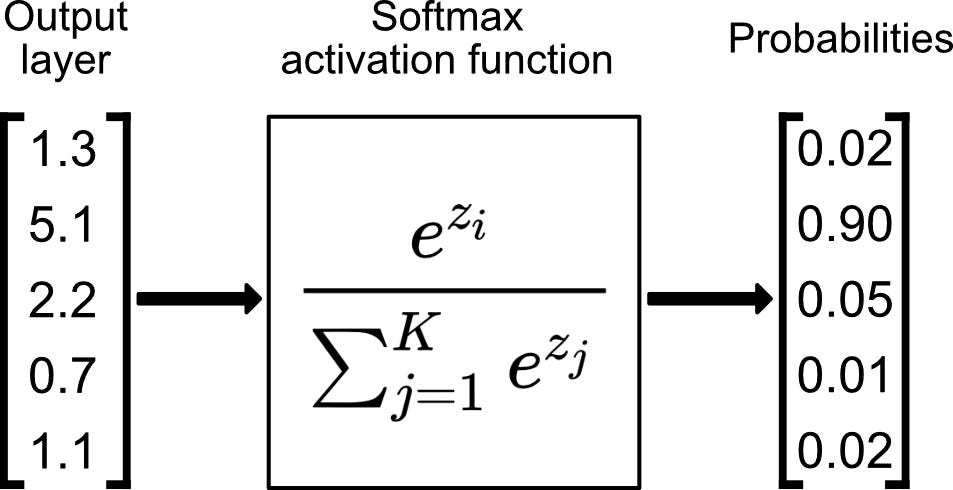
\includegraphics[width=0.450\textwidth]{Immagini/Generiche/funzionamentoSoftMax.jpg}
    \caption{Illustrazione del funzionamento della softmax \cite{ActivationFunctions_MEDIUM}.}
\end{figure}
\newpage
Come si può intuire, la somma di tutte le probabilità è uguale a 1. In altre
parole

\[
    \sum_{i=1}^{K} \frac{e^{z_i}}{\sum_{j=1}^K e^{z_j}} = 1
\]

% La derivata della funzione Softmax è complessa e viene calcolata come:
% \[
%     \frac{\partial f(x_i)}{\partial x_j} = f(x_i)(\delta_{ij} - f(x_j)),
% \]
% dove \(\delta_{ij}\) è il delta di Kronecker.

\section{La Cross-Entropy}
Un altra funzione di attivazione largamente utilizzata per problemi di 
classificazione è la \textbf{Cross-Entropy (Entropia crociata)}
\cite{GradientDescent_NeuralNetworks,ALL_DEEP_LEARNING}. 

Il concetto di cross-entropy affonda le sue radici nel campo della teoria 
dell'informazione, dove l'entropia dell'informazione, nota anche come entropia 
di Shannon, fu introdotta formalmente nel 1948 da Claude Shannon in un articolo 
intitolato “A Mathematical Theory of Communication”. La Cross-Entropy si basa sul 
concetto dell'entropia, che calcola il grado di casualità o disordine di un sistema. 
Nel contesto della teoria dell'informazione, l'entropia di una variabile casuale $X$
è l'incertezza media, la sorpresa o l'informazione inerente ai possibili risultati. 
In parole povere, misura l'incertezza di un evento.

\begin{equation}
    H(X) = - \sum_{i=0}^{n}  p(x_i)\cdot \ln(p(x_i))
\end{equation}

Maggiore è il valore dell'entropia, H(x), maggiore è l'incertezza della 
distribuzione di probabilità, mentre minore è il valore, minore è l'incertezza.
Ovvero, più è alto il valore dell'entropia più è difficile prevedere il valore 
che assumerà la variabile casuale $X$. 
La Cross-Entropy sfrutta questo concetto per misurare la differenza tra la distribuzione di 
probabilità predetta dal modello di classificazione e i valori reali. 
Maggiore è la differenza tra i due e maggiore è la loss \cite{CrossEntropy_DataCamp, CrossEntropy_365DataScience,CrossEntropy_Wikipedia}.
Per problemi di classificazione binaria la cross-entropy, definita in questo caso 
anche come binary cross-entropy, è così definita 
\cite{CrossEntropy_DataCamp, GradientDescent_NeuralNetworks}:

\begin{equation}
    C(w, b) = -\frac{1}{N}\sum_{i=1}^{N}\left[y_i \ln(a_i^{(L)}) + (1-y_i)\cdot \ln(1 - a_i^{(L)})\right]
\end{equation}

La binary cross-entropy è comunemente utilizzata nelle reti neurali con una 
funzione di attivazione sigmoide nello strato di uscita.
Mentre per problemi di classificazione su più classi, la cross-entropy, chiamata in 
questo caso anche come categorical cross-entropy, è definita come:

\begin{equation}
    C(w, b) = -\sum_{i=1}^{N}\left[y_i \ln(a_i^{(L)})\right]
\end{equation}

La categorical cross-entropy è comunemente utilizzata nelle reti neurali con una 
funzione di attivazione softmax nello strato di uscita. Minimizzando la perdita, 
il modello impara ad assegnare probabilità più elevate alla classe corretta e a 
ridurre le probabilità per le classi errate, migliorando l'accuratezza.

%\section{Il Dropout}